\documentclass[10pt,a4paper,openany]{book}
\usepackage[english]{babel}

\usepackage[utf8]{inputenc}
\usepackage[a4paper]{geometry}
\usepackage[T1]{fontenc}
\usepackage{titling}
%\usepackage{showframe}
\usepackage{graphicx}

\usepackage{tcolorbox}
\tcbuselibrary{skins}
\newtcolorbox{warning}{colback=red!5!white, colframe=red!75!black, fonttitle=\bfseries, title=Attention !}
\newtcolorbox{notice}{colback=blue!5!white, colframe=blue!75!black, fonttitle=\bfseries, title=Notice}

\usepackage{listings, multicol, color, fancyhdr,lastpage}
\usepackage[font=small,format=plain,labelfont=bf,up,textfont=it,up]{caption}
\usepackage[hyperindex=true,colorlinks=true,breaklinks=true,linkcolor=blue]{hyperref}

\usepackage[font={large,itshape}]{quoting}

\pagestyle{fancy}
\fancyhead[LE,RO]{\leftmark}
\fancyhead[LO,RE]{}

\lstset{
	language=bash,						% le language par défaut
	title=\lstname,						% on donne le nom des fichiers inclus
	basicstyle=\ttfamily\normalsize,	% la fonte de base: brute d'imprimerie
	frame=leftline,	% une ligne à gauche
	rulecolor=\color{black},	% if not set, the frame-color may be changed on line-breaks within not-black text (e.g. commens (green here))
	framerule=2pt,
	%framexleftmargin=10pt,
	keywordstyle=\color{blue},	% keyword style
	commentstyle=\color{gray},	% comment style
	stringstyle=\color{mauve},	% string literal style
	escapeinside={\%*}{*)},		% if you want to add a comment within your code
	morekeywords={*,...},		% if you want to add more keywords to the set
	morecomment=[l]{\#},
	belowskip=10pt,
	aboveskip=0pt,
	xleftmargin=25pt,
	belowcaptionskip=0pt,
	abovecaptionskip=0pt
	}

\definecolor{dkgreen}{rgb}{0,0.6,0}
\definecolor{gray}{rgb}{0.5,0.5,0.5}
\definecolor{mauve}{rgb}{0.58,0,0.82}

% fonte
\renewcommand{\familydefault}{\sfdefault}
\renewcommand{\labelitemi}{$\bullet$}


\title{\scshape Cipher'in' Letters}
\author{Stéphane 22Decembre Guedon}
\date{13 mai 2015}

%\pretitle{\centering}
%\pretitle{\begin{center}}

\pretitle{\begin{center}\Huge}
	
\posttitle{\\
		\Large\emph{Protect your online communications\\and other aspect of your life on the internet\\}
		\vspace{5mm}
		\LARGE\emph{GnuPG and OpenPGP for everybody\\}
	\end{center}
		}

\preauthor{\centering
	    \vspace{5mm}
		
\includegraphics[width=0.9\textwidth]{./images/logo-gnupg}
		\vspace{1cm}
		\newline
	}

\postauthor{
	 \vspace{5mm}\\
		}

\predate{\begin{center} version 1 of }
	
	
\postdate{\end{center}}
	

\begin{document}
	%\makeatletter
	\maketitle

	%\frontmatter
	\chapter{Preamble}
	
	This document uses my texts from my GPG-Howto or tutorial. It is the \textit{short} version, with the functions that I think are the most important in GnuPG and OpenPG.
	
	This How-to can be read on my website\footnote{english version: \url{http://www.22decembre.eu/category/howto-gpg.html}}. I wish you read, share and reshare this work, online (html) or off-line (this pdf).
	
	Of course, the texts have been slightly modified to correspond to their current form: a mini-book. But I kept the exercises from the blog articles.
	
	The aim of this document is to push internet users, so actually some big pat of the occidental population, to protect their communications in the form of mails and instant messaging.
	
	As I am writing this book, some laws, extremely dangerous for privacy and public liberties, are being voted or adopted by several european countries. I think obviously of France, but also UK or Switzerland !
	
	This pdf file has been signed by my gpg key and the tutorial's one. Those two keys have been included in the pdf itself.
	
	Here are their fingerprints:
	
	\begin{center}
		\oldstylenums{30CF 1DA5 7E87 6BAA 730D E561 42E0 A02E F1C9 35A4}
	\end{center}
	\begin{center}
		\oldstylenums{F6B2 DCE3 B6F6 A972 FF3A 1C9B 2041 3A8E 7F36 CE55}
	\end{center}
	
	The text of this document (my actual work) is under Creative Commons BY licence. I used some illustrations from external sources:
	\begin{itemize}
		\item The GnuPG logo, under CC-BY-SA licence\footnote{\url{http://www.gnupg.org}}
		%\item l'illustration de la gpg cheat sheet, sous licence CC-BY-SA\footnote{text}
		\item The comic from XKCD about password strength, under CC BY-NC 2.5 licence\footnote{\url{https://xkcd.com/936/}}
		\item The shadow of Justice, under CC BY-NC-ND 2.0 licence.\footnote{\url{https://www.flickr.com/photos/jmtimages/3286566742/}}
	\end{itemize}
	
	The sources of this document, in \LaTeX are available in the github  … . La version actuelle est … commit signé avec ma clé gpg.
	
	\tableofcontents
	\chapter{Why you should use GPG ?}

When I send emails or give my business card to people, I am continually
asked: What's GPG ? What is this file in your mail ?

\begin{figure}[htbp]
\centering
\includegraphics{\{filename\}../images/visiting.jpeg}
\caption{}
\end{figure}

I am surprised that after
\href{http://en.wikipedia.org/wiki/Global_surveillance_disclosures_\%282013\%E2\%80\%93present\%29}{Edward
Snowden's disclosures about ongoing global surveillance} by secretive
American agencies (CIA, NSA\ldots{}), and the overwhelming power these
secret agencies have, there are still many people - \emph{most poeple},
in fact ! - that don't know about GPG or personal privacy tools.

\subsection{What I am going to tell you}\label{what-i-am-going-to-tell-you}

Unlike the majority of tutorials over the web about GPG, I am going to
teach you on an incremental way, so it's easier for you to understand.

My purpose in doing this is to ensure that you know what you need to
know so that you're well-prepared by the time you need to use GPG in
practice.\\If you aren't well-prepared, it's easy to make a mistake that
renders the privacy GPG can offer you useless.\\So, we'll go one step at
a time to make sure you understand the whole thing and to allow yourself
to dive deeper at your own pace.

\subsection{What's GPG ?}\label{whats-gpg}

\subsubsection{In the beginning, there was
PGP}\label{in-the-beginning-there-was-pgp}

PGP stands for \emph{Pretty Good Privacy}.

PGP is the original software, designed by
\href{http://philzimmermann.com/EN/background/index.html}{Philip
Zimmermann}, whose goal was
\href{http://www.philzimmermann.com/EN/essays/WhyIWrotePGP.html}{defending
privacy, individual liberties and more largely democracy}.

PGP is, first and foremost, a tool to encrypt, authenticate, and protect
the contents of your email messages. This process uses a lot of
high-level math, but don't worry, because all of the math is done by the
software itself.

\subsubsection{Then OpenPGP}\label{then-openpgp}

Then the IETF (Internet Engineering Task Force) standardized PGP format,
leading to OpenPGP which made possible for every email user to exchange
encrypted emails with any other user, regardless of which email service,
program, or provider they were actually using.

\subsubsection{Finaly came GPG}\label{finaly-came-gpg}

This allowed free-softwares advocates and developers to write a
software, \href{https://www.gnupg.org/}{GnuPG} (the ``GNU Privacy
Guard''), reduced to GPG, which implement OpenPGP.\\In other words :
with OpenPGP, GnuPG and PGP users can write and send mail to each other
without any problem.

\subsection{Why would you want to use GPG ?}\label{why-would-you-want-to-use-gpg}

Are you in a couple ? Your partner send you hot pictures to make you
horny, or you simply exchange hot talks you don't want anyone to read ?

You have a cooking competition and want to share your recipe for tarts
with Bree Hodges, but not with Katherine Mayfair ?

You want to have your own business or are already working in a company
and wish to discuss matters with your associates privately ?

You are a journalist and have to communicate with your sources in a safe
way ?\\This case is very special, because ideally, your sources need to
feel confident that they can write to you in a way no one else can
overhear even before they know you.\\It is important to notice that this
was Edward Snowden's case : he used PGP and asked his contacts to do the
same to insure safe exchanges.

Some of these reasons seem shallow.\\But if we have learned one thing
from \emph{Desperate Housewives} and people surrounding us, it's that no
matter how shallow or stupid it may seem, someone might want to open
your mail and will use any measures they can to do it !

But let's switch to something else. Ooooohhhh yeeesss
\ldots{}\\\href{http://www.huffingtonpost.com/2014/04/15/gmail-ads_n_5149032.html}{Google},
\href{http://motherboard.vice.com/read/looking-up-symptoms-online-these-companies-are-collecting-your-data}{Yahoo}
and \href{https://tosdr.org/\#microsoft}{Microsoft} (Live and Hotmail
for example) all read your email to create a profile about you, a
dossier used to target advertisements, and worse.

Do you remember
\href{http://www.theguardian.com/world/2014/sep/01/nude-photos-of-jennifer-lawrence-and-others-posted-online-by-alleged-hacker}{the
fappening} ? The celebrities whose private, revealing photos have been
stolen. Do you feel their reaction sane ? If so, why don't you value
your own privacy the same ?

Good news eventhough,
\href{http://www.ginjfo.com/actualites/politique-et-economie/espionnage-nsa-depose-les-armes-devant-certaines-solutions-cryptage-20141230}{apparently
GPG is still safe} !

The thing you have to realize is that digital mail is not like sending a
letter.\\It's more like sending a postcard. Anyone who looks can read
the contents. They don't have to open a sealed envelope to do it.\\So
you can think of GPG as the envelope inside of which you put the
contents of your message. No more easy to read, intercept, or hijack
postcards!

\subsection{But, Doctor, is it painful ?}\label{but-doctor-is-it-painful}

Let's say that encryption is not the easiest task on Earth. But I see no
way or reason not to use it !

This is the reason I wrote this serie of articles; to familiarize you
with GPG so that you, too, will see no reason not to use it.\\In the
following days, I will publish regularly articles aimed at gradually
giving you the skill to master this privacy tool.

By providing you a permanent documentation, by teaching you, gradually,
to discover OpenPGP, I hope to allow you to protect your privacy and the
privacy of person's you love.

You will see that after some training, using these tools is actually
pretty easy and you do it in a natural way.

	\chapter{Is there any other way than using GPG ?}

\emph{NB : This article is much targeted to people with a special
interest in IT technology itself as an overview of secure communication
alternatives to GPG.\\Don't worry if you feel like this part is too
complicated or like it's going over your head. You can safely skip this
part or come there later when you understood more.}

So, here we are. We have OpenPGP and its software implementations, PGP
and GPG, which are tools to protect your mail from unwanted lookup. But
is it the best way ?

\subsection{Bitmessage}\label{bitmessage}

Let's take a look at \href{http://n0where.net/bitmessage/}{Bitmessage}
first. In my opinion, this is the perfect anti-example because it does
not respect the
\href{\{filename\}../Informatics/paradoxe-moquette-en.md}{carpet
paradox} : the addresses look like strings made out of random
characters, so they're a real hassle to exchange to your pen pals.

Even give your address on a piece of paper could be risky because your
friend may make a mistake while copying it. Like so easy to send your
message to someone else now !\\I think the best way to share a
Bitmessage address is to publish your address on a website you
control.\\However, even if you take this route, you still have to be
careful.

The foundation of Bitmessage itself is easy to understand, but as soon
as you dive deeper into it (a task I think is really important when
talking about safety protocols), you it gets confusing rather quickly.

\subsubsection{Some reflections on Bitmessage\ldots{}}\label{some-reflections-on-bitmessage}

One unusual thing about Bitmessage that comes to mind is the way it uses
P2P technology. The Bitmessage protocol works by sending a given message
to everybody in the network.

This makes it really less efficient with the energy. But it's also now
trivial for attackers like the NSA (the group hackers are typically
trying to escape from) to create their own Bitmessage address, collect
every message sent on the network and try to decrypt it because
apparently, it's
\href{http://www.nytimes.com/2013/09/06/us/nsa-foils-much-internet-encryption.html}{what
it already does} !

Instead of sending messages only to the recipient, the Bitmessage
protocol relly entirely on SSL/TLS cryptography to ensure privacy ! Not
the safest, as I will explain later.

\subsubsection{GPG or Bitmessage ?}\label{gpg-or-bitmessage}

\emph{This is my opinion, my use of computing tools. This is not some
sacred words to respect at all cost. A debate is possible. If you want
to troll or whatever, feel free, but without me !}

Given my above reflections, it's probably no surprise I prefer to use
GPG rather than Bitmessage. Mail is a widely recognized communications
channel, and even though I have ``no reason to hide'' - except privacy
concerns - I do understand that other people have motivations to want to
do so.\\This is especially true for those who want to hide who they are
writing to.

Use of Bitmessage marks me as a high-level \emph{hacker}, which I am
not. I can barely pretend to be a \emph{little} hacker or a
\emph{padawan}. Besides, using Bitmessage would further encourage people
to watch my email.

On the other hand, using signed or encrypted email, I still assume my
mail is being watched but I'm also able to protect it, along with my
privacy and the privacy of others. Since it is still plain email, many
more people can still use it for many more day-to-day purposes, without
learning whole new systems and while still being protected. Plus, the
more I use GPG, the more my use of it encourages other people to use
GPG, too.

And if an attacker wants to decrypt my mail, all they'd learn about me
is that I exchange thoughts with my lesbian friend, or some proposals
that I'm developing at work. Basically, useless stuff for NSA \& Co !

That said, there is a bonus: encrypting my mail is easy and takes no
extra effort on my part, but decrypting it does. Our Big Brother friends
have to spend enormous efforts and waste countless hours of CPU cycles
to decrypt things.

\begin{quote}
And make worse the life of others you don't like is really enjoyable !
\end{quote}

\subsection{Other classic email enciphering schemes}\label{other-classic-email-enciphering-schemes}

Another standard for encrypting and authenticating email is the S/Mime
standard, which uses SSL/TLS certificates very much like those used by
websites for encrypting Web traffic. Some entities and service providers
even offer free certificates for personal use.

It is the case of DanID, who mounted the authentication system NemID,
used by the danish governement and banks. It is valid to sign and
encrypt mail as well as authenticate on some websites, for example
\href{http://www.dba.dk/}{DBA}, the danish ebay, but you can't use it to
secure your website, sadly.

There's much to be said for a nation-wide system of secure certificates
like NemID, which are one step towards a digital citizen ID card, after
all. But the SSL/TLS protocol on which it is based have had numerous,
well-known problems lately. There's widespread concern that the NSA
(along with some other agencies) have been able to compromise the
certificate infrastructure or even break some of its crypto algorithms.

Personally, I tend not to trust TLS too much, because the more we look
at it, the more holes we see in it.

\textbf{\emph{Yet, I still recommand TLS use in web browsing ! A weak
shield is better than no shield at all !}}

SSL/TLS and GPG are a slightly different implementation of the same
principle : asymetrical cryptography, with a public and a private key.
But actually, I don't believe it to be easier and certainly not safer to
use SSL/TLS.

\subsection{Back to GPG}\label{back-to-gpg}

GPG tries to respect the carpet paradox: it uses well-known, easy to
understand protocols (the standard email protocol itself).\\The keys can
be identified by the mail address, or the fingerprint, easy to search
and giving a good feeling of security to users.

And, evidently, it's not been broken yet!
	%\mainmatter
	\chapter{Softwares installation}

Let's do some actual stuff : install the softwares.

\subsection{What we need}\label{what-we-need}

To use GPG you need\ldots{}

\begin{enumerate}
\def\labelenumi{\arabic{enumi}.}
\itemsep1pt\parskip0pt\parsep0pt
\item
  GPG
\item
  A keys manager like :

  \begin{itemize}
  \itemsep1pt\parskip0pt\parsep0pt
  \item
    Kgpg/Kleopatra
  \item
    Enigmail
  \end{itemize}
\item
  A mail software like :

  \begin{itemize}
  \itemsep1pt\parskip0pt\parsep0pt
  \item
    kmail
  \item
    Thunderbird
  \item
    Evolution
  \end{itemize}
\end{enumerate}

Often, keys managers are add-ons or plugins to mail softwares. They have
pretty much the same options. Choosing one other the others is just a
matter of personal preferences.

Kgpg is a part of KDE, mostly used with Kontact and Kmail. Same,
Enigmail works with Thunderbird.

\emph{The Samsungs devices with Android are now shipped with all the
correct tools including GPG. You can use and create keys with it.\\The
problem is that you can't really trust the hardware nor the software. I
think it's a good idea to just begin. After that, you might want to set
new keys using a true computer.}

By the way, you can also setup a personal mail server.\\It becomes
available to the non-computing guy with
\href{https://yunohost.org/}{YunoHost} for example.\\Or in another way,
OpenBSD, really easy to install, yet a bit difficult to master. But, as
I manage both systems now, I can tell it's not harder than a Debian!

\subsubsection{Recommendations}\label{recommendations}

\begin{quote}
Much of these recommendations are for general use, not only GPG.
\end{quote}

You ought to avoid webmail. Webmail is a bad thing, as you access your
mail through the web, so we can't ensure of safety, without even
thinking of GPG itself!

You also ought to avoid fetching softwares on third-parties websites but
rather on the author's one, or an official website like Apple's one in
case of you being a MacOS user.

When you can use free or open-source software, please do so. It's even
more important in critical protocols like security ones. Being open, the
code can be read by anyone and anybody can tell that there's no
backdoors or bad habits.

An \emph{opensource} code means that you can trust it to \emph{protect
yourself, and your privacy with it} ! And if you're really a paranoiac
(your right) then you can take code cursus and then do this checking
yourself!

When installing or setting a software, don't hit ``enter'' all the time.
Check the options. It is frequent that an install program contains a
toolbar or something else you did not ask nor need.

These micro add-ons are one of the main source of your computer being
slow, buggy, and can contain viruses or spy softwares.

Some software writers sign their binaries (the file to download) with
their GPG key or indicate MD5 or SHA1 sums.

I have not told you yet how to check these signatures, but if you know
how to do it, please do!

Encrypting and signing mail does not protect you from viruses ! They
warrant that your mail is authentic and/or has not been read by anyone
but the recipient.

\subsection{GPG}\label{gpg}

\subsubsection{Linux and co}\label{linux-and-co}

Gpg is somewhat a standard in any GNU/Linux distribution. If you don't
have it already, it means your distro is that weird I even don't know
much about it, nor its packaging tool ( \emph{Slitaz} ? )

Under Debian \& co, if not already installed - which would be really
weird, as Debian uses gpg to sign and check its softwares packages (!) -
it is it:

\begin{verbatim}
apt-get install gnupg gnupg2
\end{verbatim}

The second release is the recommended one currently.

No matter, it's in the general dependencies of all key managers we'll
see later.

Users of other distros or graphical tools like Synaptic, Apper or Muom
will simply make a research about \textbf{gnupg}. Much chance is that
your package manager tell you it's already there.

It's also in BSD base, like on OpenBSD.

\subsubsection{Windows}\label{windows}

This is a big one !

You need \href{http://www.gpg4win.org/download.html}{Gpg4win - take the
one on the top, unless you know what you're doing}, which
\href{http://www.gpg4win.org/about.html}{actually contains all the
needed softwares} : keys manager, mail client\ldots{}

Windows users, you have an easy life !

As soon as the installer is downloaded, launch it. It will propose you
to install GPG and other softwares.

\begin{itemize}
\itemsep1pt\parskip0pt\parsep0pt
\item
  GPA is a keys manager.
\item
  Kleopatra is another keys manager.
\end{itemize}

You need one of them. Kleopatra is the most documented on thee web, so I
recommend it. I use it from time to time and if you need help, it will
be easier for me if you use this one.

\begin{itemize}
\itemsep1pt\parskip0pt\parsep0pt
\item
  GpgOL, Outlook plugin
\item
  GpgEX, Windows files explorer plugin.
\end{itemize}

Install them if you want or need.

\begin{itemize}
\itemsep1pt\parskip0pt\parsep0pt
\item
  Claws-Mail, lightweight mail client
\end{itemize}

\subsubsection{MacOS}\label{macos}

Thunderbird is available on Mac and the native mail client can also
support encryption.

You need \href{https://gpgtools.org/}{Gpg pour Mac}. Please download the
Gpg Suite.

You can (actually you \emph{should}) check dmg file integrity by going
in your Downloads repository (I suppose here it's called
\emph{Downloads}) with your Terminal:

\begin{verbatim}
cd Downloads
openssl sha1 GPG_Suite…
\end{verbatim}

Typing filename, you can use auto-completion : use tab key, the terminal
will complete the filename itself.

The ssl command will generate a string of characters which have to
correspond to the one indicated on the website, just under download
button. If it fails, bare download again.

So you can install now. Open the dmg file and select the correct
options. You need \emph{MacGPG2}, \emph{GPGPreferences}, \emph{GPG
Keychain Access}.

If you use \textbf{Mail}, the native client, you need \textbf{GPG for
Mail} but if you use Thunderbird, you need \textbf{GPG Services}.

\subsection{A mail client}\label{a-mail-client}

\begin{quote}
I won't describe mail and address configuration. If you came there, I
believe you're motivated to learn/search the solution yourself or you
already know how to do it.
\end{quote}

\begin{quote}
Yet, one can still \href{\{filename\}../pages/contact.md}{contact me} to
ask for help and a basic tutorial for setting Thunderbird is available
\href{https://support.mozilla.org/en-US/kb/new-email-address}{there}.
\end{quote}

So, you have the base software, but nothing else currently. Choose your
mail client.

\subsubsection{Thunderbird}\label{thunderbird}

Thunderbird is available for downloading
\href{https://www.mozilla.org/en-US/thunderbird/}{there} (link for your
language and your operating system).

It is also available in Debian under the name Icedove due to
\href{http://en.wikipedia.org/wiki/Mozilla_Corporation_software_rebranded_by_the_Debian_project}{the
Mozilla-Debian issue}.

So you can install it with apt:

\begin{verbatim}
apt-get install icedove
\end{verbatim}

\subsubsection{Kmail and Evolution}\label{kmail-and-evolution}

Kmail is a part of KDE, Evolution is a part of Gnome. So if you are
under GNU/Linux, you should use your favorite package manager.

\begin{verbatim}
apt-get install kmail

apt-get install evolution
\end{verbatim}

Same as before : Synaptic or other graphical installers will setup all
dependencies, including \textbf{gnupg} if for some weird reason it's not
already the case.

\subsubsection{Claws-Mail}\label{claws-mail}

If you are on Windows, remember that the Gpg4win installer proposed you
to install as well \textbf{Claws-Mail}.

\subsubsection{The others}\label{the-others}

There is a \href{https://windows.kde.org/}{Windows version of KDE}, but
I never tried to use it - I feel already really fine on GNU/Linux and
don't see why I should change that.

Sylpheed, mail client available under Linux distributions, Windows, Mac
and other Unix.

\subsection{A keys manager}\label{a-keys-manager}

\begin{quote}
To remind you : You need only one of these softwares. Often the choice
much depends on your environment (operating system).
\end{quote}

\subsubsection{GPG Keychain under Mac
OS}\label{gpg-keychain-under-mac-os}

The keys manager is named GPG Keychain under Mac Os and you have already
installed it normally when you installed Gpg for Mac.

\subsubsection{Thunderbird : Enigmail}\label{thunderbird-enigmail}

\textbf{\emph{The same day this article was published, Enigmail released
a new versionas well : 1.8.1. You should use this new one as it is much
more usable.}}

If you use Thunderbird, you will need Enigmail, which is actually a
plugin used by Thunderbird to interact with Gpg.

\paragraph{First way : Downloading on the
website}\label{first-way-downloading-on-the-website}

Installation here is the same as a Firefox module : xpi.\\You need to
download the module \href{https://www.enigmail.net/download/}{there} and
of course take the one corresponding to your operating system.

The xpi extension setup as described there : you need to launch
Thunderbird, select «Tools» in the menus bar on top, then
«add-ons»,«plugins», «extensions» or «modules».\\Or, depending on your
version of Thunderbird, select the big button on top and right and
select «add-ons».

Here, you can tell Thunderbird that you want to install a plugin
clicking on the bottom left on «install\ldots{}». Thunderbird will ask
you where you downloaded the xpi.

\paragraph{Second way : Install with Thunderbird
itself}\label{second-way-install-with-thunderbird-itself}

You can ask Thunderbird to install it itself.

Like previously, go to the add-ons window and make a research about
Enigmail. The software should appears on top of the list with an install
button.

Once you installed the plugin, you need to reboot Thunderbird itself.
That's it.

\paragraph{Debian Bonus : installation via
Apt}\label{debian-bonus-installation-via-apt}

If you use Icedove (sic !) you can also install Enigmail with apt. It is
good if you share your computer with other users.

But if you do it this way, take care when upgrading : don't upgrade on
Mozilla request but bare wait for Debian to update it!

If you wish to use another release than the one in Debian apt store,
uninstall it using apt before.

\textbf{\emph{One only release of this software per machine ! I believe
it to be a safety mesure.}}

\begin{verbatim}
apt-get install enigmail
\end{verbatim}

\emph{NB : If Debian did it, why not others like Mageïa or Arch ? Try to
find Enigmail in your packages manager.}

\subsubsection{Kgpg/Kleopatra}\label{kgpgkleopatra}

Kgpg and Kleopatra are two softwares used to manage keys and
certificates in KDE. I prefer to use Kgpg, but it's still useful to have
both installed.

If you are a KDE fan like I am, then chances are that they are already
there.\\Else, as previously :

\begin{verbatim}
apt-get install kgpg kleopatra
\end{verbatim}

Remember, if you are under Windows, you got Kleopatra in Gpg4win
installer.

\subsubsection{The others}\label{the-others-1}

Under Gnome, you have Seahorse, which I don't know at all. I doubt that
it is really different from Kgpg. Available under Debian :

\begin{verbatim}
apt-get install seahorse
\end{verbatim}

\subsection{What's next ?}\label{whats-next}

And it's all for now. As said, I intends to do it progressively. In the
next article, I introduce the \href{\{filename\}3-logic-en.md}{logical
side} of GPG.

	\chapter{A slice of theory and logical}

Let's move on to the logical side now.

\section{OpenPGP, how does it work ?}\label{openpgp-how-does-it-work}

OpenPGP uses asymmetric cryptography, also called public-key cryptography. When talking about GPG keys, we actually talk about couples of keys : a public, and a private key.

\section{Does it have to be that complicated ?}\label{does-it-have-to-be-that-complicated}

When you sign a mail, you want to insure your pen pal that it's truthful. Same as seals in the Middle-Age : the seal's wax warranted
message's inviolability.\\
\\
You have to sign your message with something you're the only one to
possess : your \textbf{\emph{private}} key !\\
\\
And how do your pen pals would check this message is authentic ? With something that is well-known, available to anyone : checking signatures
is done with your \textbf{\emph{public}} key !\\
\\
Opposite, when one encrypt (or cipher) a message, one wants to protect it. You are the only one who should be able to read it with something
you are the only one to possess : your \textbf{\emph{private}} key !\\
\\
But as anyone should be able to send you encrypted mails, the ciphering operation should be done with something available to anyone : your
\textbf{\emph{public}} key !

\section{Be cautious !}\label{be-cautious}

A signed mail \textbf{can be read by anybody online}. Just like a random mail actually. The signature warrant that you are the true sender and that it has not been altered. So a signed mail has more juridical value than a
non-signed mail.

\section{Summary}\label{summary}

We sign mail with \emph{private} key. We check signed mail with the sender's \emph{public} key.\\
\\
We encrypt mails with the recipient \emph{public} key, and they decrypt with their \emph{private} key.\\
\\
It's always the same side of the liaison that uses the same side of the key: you will always (or almost) use your private key, and your pals
will always use your public key.\\
\\
Your private key should be protected like Precious\ldots{}

\begin{figure}[htbp]
\centering

\includegraphics{./images/gollum.jpg}
\caption{}
\end{figure}

It allows you to control your side of the liaison, to prove your identity and read your mail !
	\chapter{Create and export your keys}

Let's go ! You're going to do your first real action to use GPG :
generate your first key. Or more exactly, your first key pair. Remind
that every GPG key has actually two sides : a public and a private side.

\textbf{This chapter might look long, but it's an important one. Creating keys takes a few minutes and you have almost nothing to do. So
please, take your time.}

\section{Notice}\label{notice}

NB : for those who are affraid, or concerned about privacy, that I gather a lot of mail addresses, it's no big deal to me that you use a
fake address for your mail and keys. After all, it's what I do with the tutorial's address. At the end of the tutorial, you can create a new key on your real address, follow again all the various steps. But you won't send it to me: instead, you will use it for real ! And I am happy of that !

\section{Let's generate the key.}\label{lets-generate-the-key.}

Open your keys manager : Kgpg, Kleopatra or Enigmail (or another
one\ldots{}) and look for the option to create new keys.

\begin{description}
	\item[Kleopatra\footnote{link to the documentation \url{https://docs.kde.org/stable/en/kdepim/kleopatra/index.html}} :] \emph{Files \textgreater New certificate\ldots{} \textgreater{} Create a personal OpenPGP key pair}

\item [Kgpg\footnote{link to the documentation \url{https://docs.kde.org/stable/en/kdeutils/kgpg/}} :] \emph{Keys \textgreater{} Generate key pair}
\item [Enigmail (inside Thunderbird itself) :] \emph{Enigmail \textgreater{} Key Management}. Then select \emph{Generate \textgreater{} New Key Pair.}

\end{description}


\subsection{Which address to indicate}\label{which-address-to-indicate}

The software will ask you which address to use with your key.

You can actually set several addresses on a key, but now, better not to do complicated and set just one.

\subsection{Key type}\label{key-type}

Perhaps you will be proposed several algorithmes : DSA \& ElGamal, RSA or RSA and RSA. Choose RSA and RSA. It is the strongest combinaison and allows to sign and encrypt. In Enigmail (tab \emph{advanced}), you'll simply choose RSA.

\subsection{Key size}\label{key-size}

It will ask for a size : 1024, 2048 or 4096 bits. Basically, the larger the key size, the stronger the key, the longer it is to create the key.
The software will then request to your operating system's \emph{random generator} some \emph{entropy} of this size.

\begin{notice}
I must admit that I don't understand the whole thing there. As soon as I
try to figure out this entropy, entropy size, I am out ! But I
understood very well that, the more entropy you have, the stronger the
key !
\end{notice}

Today, 4096 bits is the recommanded value. The key generation will take some time. You mustn't worry or stop the
software. You can reduce this time using your computer ! The more you use your computer (particularly hard drives access, called \emph{I/O access} in
geek jargon), the more you generate entropy for your key ! Isn't that fun ? The good is then to update/upgrade your Linux distribution (high
use of the hard drive).

\subsection{Time expiry}\label{time-expiry}

It's a good idea to set a time expiry. If you loose access to your key, it will be marked invalid after the
alloted time. What I do is set a one year validity, and around one month before, push
it away to one more year.

\subsection{Passphrase}\label{passphrase}

A \emph{passphrase} is a really long password. For example fifteen or
twenty characters. There is several methods to create a strong password.

\begin{figure}[h]
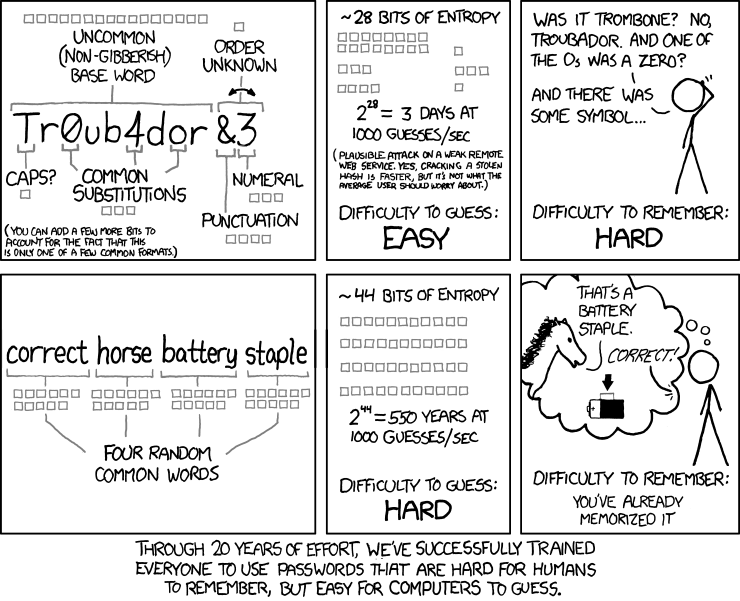
\includegraphics[width=\linewidth]{./images/password_strength.png}
\caption{What a strong password should be, by XKCD (\url{https://xkcd.com/936/})}
\end{figure}

\emph{Bonus for foreigners} : Use a pretty complicated word of your own
language to start your password. This way, surrounding humans may have
problems finding it !

What I do is that I take a word in my immediate environnement or a
concept that I think of, and then I replace characters in : A becomes @,
l becomes 1 or !, I add numbers\ldots{} One or two changes like this and
the password is strong enought.

\subsection{What for a passphrase ?}\label{what-for-a-passphrase}

You can choose not to set a passhprase. I must admit I did not do it for
long. Today I do and recommend it. It simply adds another security. If you are not the only one to use your computer, or if you use GPG on
your phone or your tablet (often unlocked on the table) then you ought
to set a passhprase.

\subsection{Revocation certificate}\label{revocation-certificate}

It is a really good idea to create a revocation certificate, and the key
manager should ask for it. In case you lose your key, corruption, or someone steal your private
key, then you just publish it on the keys servers. With the updates of
keys servers, the key is declared as invalid quite fast.

This is a safety in case you got some troubles with the private key. If you just want to change your key in a proper manner, this is not at
all the good way. I will tell you more in a future chapter.

\section{Exercise}\label{exercise}

I thought this tutorial pedagogic from the beginnig. So I am going to
make some little exercises there and now. I created a mail address on my
server for the various purpose of this tutorial, and some keys to play
with.\\
\\
\textbf{These keys will never used for anything else than this tutorial.}\\
\\
I will ask you to just send your public key to the mail address. This is
what some people do to exchange keys. Yet there are other ways, but this
topic is for the following chapters. After I received your key in mail, I will answer you saying if your keys
has the correct characteristics. I also need it for the next exercise.

\subsection{To export your key}\label{to-export-your-key}

To send me your key, you have to \emph{export} it. In order to do so, you have to ask your keys manager. You have to be carefull, as your keys manager can export the whole pair, public and private.

I ask here for your \textbf{public} key !

As said before, and as its name state it, the public key is available to
anyone. The keys manager will propose you to export your key as a
\emph{gpg} or \emph{asc} file.

This file is actually a raw text file, containing the key itself, which
is a long string of characters. You can edit it with a text editor, like
Notepad or another.

\emph{And no, Word and OpenOffice are not text editors!}

\begin{warning}
	If you open the file, don't modify it!
\end{warning}

Then send it to me as attached file in mail to \emph{Tuto-gpg @ 22decembre.eu}.

\emph{NB: Kmail (mail client in KDE) propose also in its menu
}\textbf{Attach\ldots{}} to send your own public key. So simple.	
	\chapter{Sign your mail}

So you followed the path and got a gpg key. Wonderful.

You can ask for some help on the tutorial address : \emph{Tuto-gpg @
22decembre.eu}.

Now, you will learn how to use your key with your mail.

\subsection{How to make your various pen pals use your key
?}\label{how-to-make-your-various-pen-pals-use-your-key}

\subsubsection{Config' of mail client}\label{config-of-mail-client}

First of all, you have to tell them about GPG. A little text on the
bottom of your mail will be enough. This text is called
\emph{signature}. Not to be confused with your GPG signature on your
mail itself.

Here is my English signature for example:

\begin{quote}
The file \textbf{\emph{signature.asc}} is not attached to be read by
you. It's a digital signature by GPG.\\If you want to know why I use it,
and why you should as well, you can read my article
there:\\http://www.22decembre.eu/2015/03/21/introduction-en/
\end{quote}

This text is to be filled in your mail client config'. You will set
there also your various choices for your GPG signatures.

\paragraph{Kmail}\label{kmail}

With Kmail, it's \textbf{\emph{Settings \textgreater{} Configure
Kmail\ldots{} \textgreater{} Identities}}.

There, you will find cryptography options, where you set which
\textbf{\emph{private}} key to use to sign your mails.

You will also indicate which \textbf{\emph{public}} key is to use when
encrypting mail to yourself (pretty good way to share information across
devices, like a wifi password !) About format, it is better to use
\emph{OpenPGP/Mime} rather than \emph{inline}.

It is also important to set your preference about mail composing in
\textbf{\emph{Settings \textgreater{} Configure Kmail\ldots{}
\textgreater{} Composing}}.

I checked almost everything except \emph{Always show the encryption keys
for approval}. The options are pretty well described for you to
understand if you want to use them or not.

\paragraph{Thunderbird}\label{thunderbird}

\emph{You can also read this
\href{https://support.mozilla.org/en-US/kb/digitally-signing-and-encrypting-messages}{documentation}.}

In \textbf{\emph{Tools \textgreater{} Account Settings}}, select
\emph{OpenPGP Security} under the address you want. Select the option
\emph{Enable OpenPGP support (Enigmail) for this identity} and then
\emph{Use email address of this identity to identify OpenPGP key}.

You can then choose your defaults settings : encrypt, sign or not, and
if you want to use \emph{PGP/Mime}, which I recommend.

You have also some good options to set in \textbf{\emph{Enigmail
\textgreater{} Preferences}}.

\paragraph{Evolution}\label{evolution}

\emph{Edit \textgreater{} Preferences}

Select \emph{Mail accounts}, then the needed account and click
\emph{Edit}.\\In the following account editor, go to the \emph{Security}
tab on the far right, and in the field \emph{PGP/GPG Key ID} : copy the
8 characters ID that your keys manager gave you. Remember to set your
default options.

When writing a new mail, in the \emph{Security} menu, click on \emph{PGP
Sign} and/or \emph{PGP encrypt}.

\subsubsection{Shall you sign and encrypt all your mail ?}\label{shall-you-sign-and-encrypt-all-your-mail}

This question is more of ethical nature. It is a personal choice.

Anyway, your software has certainly some big buttons that just want to
be used to realise the cryptographic operations.

I like Phil Zimmerman's thoughts on the matter:

\begin{quote}
What if everyone believed that law-abiding citizens should use postcards
for their mail? If a nonconformist tried to assert his privacy by using
an envelope for his mail, it would draw suspicion. Perhaps the
authorities would open his mail to see what he's hiding. Fortunately, we
don't live in that kind of world, because everyone protects most of
their mail with envelopes. So no one draws suspicion by asserting their
privacy with an envelope. There's safety in numbers. Analogously, it
would be nice if everyone routinely used encryption for all their email,
innocent or not, so that no one drew suspicion by asserting their email
privacy with encryption. Think of it as a form of solidarity.
\end{quote}

Remember, you can always sign all your mail. It's pretty rare that it
will cause trouble to your pen pals (mostly because they have a bad/old
email client).

\textbf{A signed mail is authentic. Your pen pal will be sure that it
comes from you and that it has not been changed on the path. But it's
still possible for everybody to read it.}

But you can encrypt your mails only if your pen pals use GPG also,
because you need their public key to encrypt mail for them.

\subsection{Exercise}\label{exercise}

Today, I am going to ask you to simply send me a signed mail. Bare
simple !

This is why I asked you to send me your key in the last article: I need
it to check your signature. Checking your signature, I can insure you
that you understood this part of the tutorial.

So, let's do it : write a mail to \emph{Tuto-gpg @ 22decembre.eu}. You
can say what ever you would like to say, send a picture, make a comment
about the tutorial, say that you love me\ldots{}

Before sending, use the \emph{Sign} option, or the button.\\If, like me,
you setted your mail software to sign all your mail, you have nothing
more to do than hitting the \emph{send} button now.

When you send me your mail, check the
\href{\{filename\}6-crypted-mail-en.md}{following} article !

I am waiting forward reading from you soon.

	\chapter{Read and write encrypted mail}

Let's go further. You will encrypt your mail. It was the first objective
of this article series. Yet, there is more to come !

Did you followed the previous steps ?

So, I must have sent you a mail. It is encrypted and you are the only
one able to read it.

\subsection{What did I do ?}\label{what-did-i-do}

When I received your public key, I imported it in my keyring.\\It
allowed me to analyze it and mail you back this answer: \emph{yes, your
key is fine}.

\subsection{Consequences}\label{consequences}

As I received your public key, I can now send you encrypted mail.

\textbf{If you received an encrypted mail, you are normally the only
person able to read it. But it does not tell you about the sender.}

But if I sign it, you can't check the signature, as you need my public
key to do so, and I have not yet told you how to do it.

\textbf{Signing a mail means that I am the true sender of it.}

This is the reason your mail software says that this mail is signed with
gpg, but it can't check the signature.

\subsection{Some little caution}\label{some-little-caution}

Be cautious. Only the main body of the mail is encrypted. The header,
subject and other meta-datas (who sent the mail, to whom\ldots{}) are
clair and readable text. It is hard or even impossible to do in another
way: how mail servers could know whose mail it is and who to give it if
destination is not available ?

Thus, it is good practice to set a neuter subject if you want to insure
good confidentiality.

Something like «a good plan» rather than «the great plan to world's
domination !» or «last production figures» rather than «prod' figures
rising by 50 \%: everything is good baby !»

\subsection{How to get the public key ?}\label{how-to-get-the-public-key}

\subsubsection{By mail}\label{by-mail}

I could have send you the public key by mail in the same way as you did.

But this is not safe: a malicious person could have hijacked your mail
and replaced your key by another.

This is the kind of thoughts I would like you to have: safety on
internet is a process, a way of thinking.

\subsubsection{On the web}\label{on-the-web}

You can place your key on a webpage if you have one. In that case, it is
good policy to indicate the fingerprint.

A key fingerprint is a series of numbers and characters unique to the
key. It allows to identify (quite safely) a key and same time insure it
of its integrity.

Your keys manager can give you this fingerprint. It looks like this :

\begin{verbatim}
30CF 1DA5 7E87 6BAA 730D E561 42E0 A02E F1C9 35A4
\end{verbatim}

This fingerprint is the one of \emph{Tuto-gpg @ 22decembre.eu} GPG key.

Same principle as \href{http://en.wikipedia.org/wiki/MD5}{MD5 sums} for
downloaded files other the net - Linux distribution iso image for
example.

Some persons also set their key fingerprint on their business card,
easier to give them.

\subsubsection{On the keys servers}\label{on-the-keys-servers}

Knowing a key fingerprint, it is also possible to find it on the
internet ! Actually, on such servers called «keys servers» or «gpg
servers».

Here are some servers:

\begin{itemize}
\itemsep1pt\parskip0pt\parsep0pt
\item
  hkp://keyserver.ubuntu.com/
\item
  hkp://pool.sks-servers.net/ NB : you will certainly visit their
  \href{https://sks-keyservers.net/i/}{website}.
\item
  hkp://pgp.mit.edu/
\item
  hkp(s)://keys.gnupg.net/
\end{itemize}

You can tell gpg which server to use first with your keys manager
settings.

The S indicate that you use the server with a secure TLS connexion. This
way, if you're a paranoiac, no one knows which keys you are searching.

These servers allow you to make your key public, find keys of people you
don't know, and finally check their mails signatures.

\subsection{Exercise}\label{exercise}

The exercise today is to find the tutorial key and send me an encrypted
mail.

\subsubsection{Find the key}\label{find-the-key}

As you understood it, the aim is to make you understand the way keys
servers work.

Open your keys manager, and then the dialog box to servers. It will ask
you for a string to search, meaning a fingerprint or a mail address.

You can copy-paste the key fingerprint or the mail address (both written
above).

Your keys manager will then show you some keys to download.

Either you wrote the mail address, and shall check the fingerprint, or
opposite, copied the fingerprint and shall check the address. I actually
created several keys, not to screw you but to make you think and work
your logic.

This tutorial aims at teach you to use GPG. So you have to use it and
confront it.

By the way, please note that these persons signed the key:

\begin{itemize}
\itemsep1pt\parskip0pt\parsep0pt
\item
  \href{http://alterlibriste.free.fr/}{alterlibriste}
\item
  \href{http://lehollandaisvolant.net/}{le hollandais volant}
\end{itemize}

They helped me in some ways, because I could use their texts, or they
encouraged me to write this tutorial.\\These other persons also helped
me:

\begin{itemize}
\itemsep1pt\parskip0pt\parsep0pt
\item
  \href{http://genma.free.fr/}{genma}
\item
  \href{https://maymay.net/}{Maymay} who helped with some of the English
  texts.
\end{itemize}

I wish to thank them all. If you want to thank me as well, feel free to
give a nice word in your mail, or some little money on the flattr button
in the left column.

Now, look at the mail I send you: your mail software might have change
its announcement!

\subsubsection{Write an encrypted mail}\label{write-an-encrypted-mail}

You have to write me an encrypted mail. You can also sign it, but it is
not the aim of this part. Do as you want.

Just before sending it, select the \emph{Encrypt} option or button. Here
it is !

Maybe your mail software even proposed you to encrypt the mail while
writing it because you now have the needed key.

Isn't it beautiful?

Hey, come to read the \href{\{filename\}7-sign-keys-en.md}{last one}!

	\chapter{Sign keys}

I wish you to be able to begin using gpg, so you need as well to sign keys, at least with your few friends or family members who read this
tutorial.

\section{Sign keys\ldots{}}\label{sign-keys}

Yes, with gpg, one can sign mails, files, and \ldots{} gpg keys !

\emph{So delicious}

When you sign a key, you grant it some credit, and you indicate it to everybody fetching your signature. Signing a key sets its owner to be legitimate. We are going to call it \emph{immediate trust links} (ITL to be short): these are all the persons that you have meet and checked ID and signed the key. Please be aware it's a concept that I define here, for practical reasons, helping you to understand.

\section{An identity problem}\label{an-identity-problem}

Let's take an example: John asks you to sign his key. You shall first verify that John is the owner of the key, so check with him the fingerprint. You shall then verify John identity, looking on his ID with a photo, but not only. Identity is much larger: it's also every other sides of a person. What function he holds in an association, blog writer, social networks\ldots{}

Everything that gives you more confidence in John's identity should be checked. As soon as this various points are validated, you are sure that it is the right key and the right person. Then you can sign it.

\section{Trust}\label{trust}

Signing a key, you also grant a trust level to the owner. These two are linked but also distinguished things, and it is important to understand it. There are five trust levels.

\begin{itemize}
\itemsep1pt\parskip0pt\parsep0pt
\item
  unknown (default)
\item
  none
\item
  marginal
\item
  full
\item
  absolute/it's my key
\end{itemize}

These trust levels indicate which confidence you have in the owner's ability to check ID and maintain their immediate trust links (ITL). And
also what confidence you have in their judgment regarding other person's behavior. For example, you can check one of your sibling's key. So you trust \textbf{\emph{that precise}} key !

But you feel that your sibling is still not fully OK with OpenPGP. Maybe he signs without much precaution, or grant a trust level too much high. So you don't trust his ITL, you sign his key but with a \emph{none} trust.

That low trust level is something you can (\emph{should} !) do without shame or fear. For that purpose, the trust level is written in the
signature in a way that it remains a \emph{private} information.

\textbf{\emph{Expressing your trust and judgment about a person is free speech !}}

The more you will respect such considerations, the more your own judgment will be respected by your peers, particularly people you know
the most, and the more your own ITL will be granted high trust value as well. I think that we should sign with a marginal trust by default and grant full trust only to people we know they behave really serious with OpenPGP. Your ITL is constituted of the keys (and their owners) that you have signed and also the trust level you have granted them.

\section{Examples}\label{examples}

You meet some people in a bar when there is a meeting of your LUG.

\subsection{Arthur}\label{arthur}

Arthur tells you that he begins using GPG and wish to build his Web of Trust. \emph{OK}. You verify correctly his identity and he does the
same to you. Then, at home, you sign his key. But you set a \emph{none} trust level, because you think he is not yet skilled enough. This \emph{none} trust level does not forbid you from asking him, one month later, how he does with it, figure of his seriousness, and raise
his trust level. This \emph{none} trust level does not forbid him as well from granting you a high or low trust level. And other people sign his key as well.
Signatures that can be positive !\\

\emph{You should not feel ashamed or disrespectful to set a low trust level to Arthur.}

\subsection{Miriam}\label{miriam}

Miriam tells you she is a Debian developer. You check her ID and key. At home, you check also her Debian dev' page. So you sign her key with a full trust level because you know Debian dev' use a lot Gpg with seriousness.

\subsection{Greg}\label{greg}

Greg tells you he uses Gpg often. After having checked his key you sign it with a marginal trust, because you have no special reason to grant more.

\subsection{Karolina}\label{karolina}

Karolina tells you she has a really good signature system, well described in a written document available on her blog (it's a
\emph{signing policy}). You decide to grant her a full trust, because of this signing policy, that you think it is well designed and fair.

\section{The Web of Trust}\label{the-web-of-trust}

What is the Web of Trust ?

The Web of Trust are all the ITL, added and set together in a complete chain:

You set a marginal trust in Greg's key, his ITL has also marginal trust.

You set a full trust in Miriam. It's like getting all her contacts directly into your trust link. And it's Miriam who defined if you
should trust this or this person that you never meet actually - because you trust Miriam's judgment. Then, if Miriam sets a person to high
trust level, then this third person also get in your \emph{larger} trust link. But it's really important to understand that you \emph{should not} sign any of the keys already signed by Miriam unless you meet the owner. Miriam did it, so your keys manager will recognize it as valid. Why would you want to sign the key then ?

Gpg will calculate which actual trust level should be granted to which key through the Web of Trust. By default, Gpg won't go farther than five trust links, and it needs three marginal trust signatures on a key to mark it valid, or one full
trust signature.

\section{What if \ldots{} ?}\label{what-if}

You have to understand clearly that the Web of Trust is to be considered seriously.

For example, political opinion, race, religion, sex nor even your social status towards a key owner should never go into consideration when
granting a trust level. Only your judgment about the owner ability to maintain its ITL is important! If you meet someone who says you he signs people with great care, with a detailed signing policy, you can greatly admire his seriousness and grant him full trust. Then in the discussion, you understand he is a neonazi pedophile who eats kittens for breakfast with Worcester sauce, you \emph{still should} sign his key !

Of course you go to the police now and then, but both actions are compatibles.

\section{Falsehood ?}\label{falsehood}

\subsection{What if someone tries to screw me with a fake key ?}\label{what-if-someone-tries-to-screw-me-with-a-fake-key}

First, signing a key, you also sign a mail address. So you have also to check it. And the most simple in that case is to ask the person to send you a signed mail using it (can be done later, no problem). That way, you are sure that you have sign the key belonging to the person you met, who owns also this mail address. Yet, it's a bit heavy. Choose to do it or not.

\subsection{One might want to write to someone unknown. How to be sure to get the right key ?}\label{one-might-want-to-write-to-someone-unknown.-how-to-be-sure-to-get-the-right-key}

It's the purpose of the Web of Trust.

If you wish to write to Valentina, and some malevolent persons engineered some fake key(s), uploaded it on the keyservers, how to be
sure to get the right one ? There are much chances Valentina's key is the one with the most signatures. And, really important, the more these signatures are
diverse (nationalities, functions\ldots{}), the safer the key will be !\\It is easy, for example, to create keys with twenty signatures on it. It is much harder (not to say impossible) to engineer a key with one or two \emph{fake} signatures from Debian dev'. And it is really easy to
have your key signed by a Debian dev' ! Not because they are \emph{easy} people. Because they are widespread. If you live in a big occidental
city, there are much chances you have a Debian dev close by, and that (s)he will sign your key (following his/her signing policy) in exchange
for a nice moment in a bar. If it's easy to create fake keys, it's also easy to make it signed and validated by a public person, with a public identity (Debian or free software dev', blog writer, member of an association\ldots{})

And when you have to choose, you will choose this last key.

\section{What is my responsibility there ?}\label{what-is-my-responsibility-there}

The Web of trust is a \emph{relative} trust system. There is no central authority, typically a State, that sets which identity is wrong or right. It's you who should judge what trust level to grant and to whom. Don't be afraid of such responsibility ! This Web of Trust is democratic: if you grant a wrong trust level, your ``ballot'' shall be balanced by others. Well documented \emph{signing policies} strengthen this democratic aspect because they are unbiased, as describe above (the neonazi eating kittens\ldots{}).

\begin{figure}[h]
\centering

\includegraphics[width=0.7\linewidth]{./images/justice.jpg}
\caption{The shadow of Justice}
\end{figure}

Responsibility is individual and distributed. It's actually P2P ! \emph{We the People} are the authority who validate keys.

\section{Exercise}\label{exercise}

OK, you understand the Web of Trust ?

I will ask you, as exercise, to sign the tutorial's key, to apply the trust you feel fine and then mail it to me. Normally, you should not do that OK ? We have not met, no Id checked performed. This is why I wrote in the early chapters the keys will be used only for the tutorial purposes.

\subsection{How do I do ?}\label{how-do-i-do}

In your keys manager, select the tutorial key, then use the \textbf{\emph{Sign}} option. The software will ask you which trust level to grant to the key. If you have several private keys, it will ask you also which one to sign with. You can also use the key properties dialog box and simply change the trust level. Signing will occur automatically.

Then you have to export it in a file, like you did before when creating it, and join this file. When I fetch it, the signatures will add to the
other signatures of the key. I will, after, mail you your own key signed with the tutorial one.

Just let you know also that KGpg (and other softwares) have an option to sign the key and mail it directly in one movement.

\subsection{Precisions}\label{precisions}

Some softwares (KGpg for example) focus on the identity checking to tell you which trust level fits best for you. It means that, as the identity
was checked fine this time, it will be done the same way later. This does not change the meaning of your signature. My statements above are still valid: the trust level granted tells about how much you judge the key owner able to maintain his/her ITL.

It is still that trust level you have to set.

These softwares have some wrong ergonomic. If you have questions, don't hesitate to read again more documentations, or to write me.
	
	\chapter{Various inspirations}
	
	\begin{description}
		\item[TED conference, from Glenn Greenwald, one of the two journalists who helped Edward Snowden:] \url{https://www.ted.com/talks/glenn_greenwald_why_privacy_matters}
			
		\item[Security in a Box:]\url{https://securityinabox.org/en/women-hrds/thunderbird/windows}
		
		\item[OpenPGP Best Practices:]\url{https://help.riseup.net/en/security/message-security/openpgp/gpg-best-practices}
		
		\item[Miriam Ruiz's blog, Debian dev, whose name I used in the article about keys signing:]\url{http://www.miriamruiz.es/}\\
		
	\end{description}
	
\end{document}